\chapter{Diagrama de classes}

A figura \ref{fig:fullDiagram} é o diagrama de classes detalhado do protótipo.
\begin{figure}
    \centering
    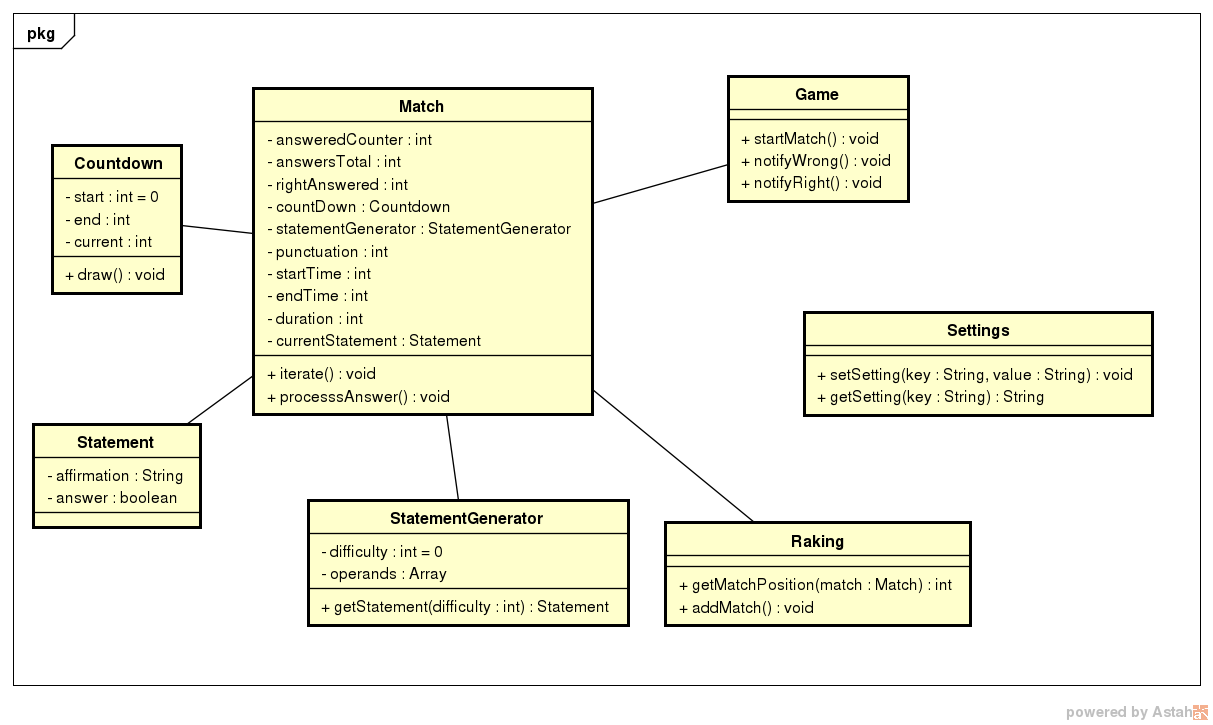
\includegraphics[width=0.8\textwidth,natwidth=610,natheight=642]{ClassesFullView.png}
	\caption{Diagrama de classes completo}
    \label{fig:fullDiagram}
\end{figure}


\chapter{Bibliotecas relevantes no desenvolvimento de jogos WEB}

A quantidade de ferramentas WEB á disposição dos usuário é
enorme. Segundo \autocite{html5mostwanted} desenvolvedores da WEB são
geralmente de mente aberta e desenvolveram uma variedade de bibliotecas
e frameworks pela internet.

Sabendo disso, é uma tarefa praticamente impossível ter habilidade
em todas as ferramentas disponíveis. Entretanto, é importante que
os desenvolvedores ao menos conheça as ferramentas mais importantes
disponíveis para que no momento necessário saibam qual aprender.

\cite{creatingFun} ressalta a importância de sermos moderados
quanto a escolha de bibliotecas no contexto WEB multiplataforma.
\begin{quote}
Muitos desenvolvedores da WEB utilizam bibliotecas como jQuery e o
Prototype de modo que se vejam livres de terem que lidar com
partes triviais do desenvolvimento WEB, como selecionar e
manipular elementos do DOM. Muitas vezes essas bibliotecas incluem
várias funcionalidades que não são utilizadas. É recomendável
cautela para verificar se realmente é necessário adicionar 50-100k
de bibliotecas, ou se alguma coisa mais simples e menor não trará
os mesmo benefícios, especialmente quando desenvolvendo
multiplataforma onde uma rápida conexão a internet nem sempre é
garantida.
\end{quote}

Esta preocupação aumenta no contexto de desenvolvimento
de jogos. Ainda segundo \cite{creatingFun} o site MicroJS
\url{https://microjs.com} oferece uma coleção de micro bibliotecas
focadas em áreas particulares em detrimento de grandes bibliotecas
cheias de funcionalidades.

\section{CSS}

A biblioteca -prefix-free \url{http://leaverou.github.io/prefixfree/}
é um polyfill que possibilita os desenvolvedores utilizarem CSS sem
a adição de prefixos, o que torna o trabalho de desenvolvedores bem
menos redundante. A biblioteca é razoavelmente leve (2KB), e quando o
sistema desenvolvido com ela estiver pronto e o CSS evoluir removendo os
prefixos utilizados, ela pode ser removida.

\chapter{CROSSWALK}

Crosswalk empacota os fontes juntamente com uma versão do Chromium, a
versão Open-source do Google Chrome. Isso faz com que o software se
comporte da mesma forma para todas as versões de dispositivos Android.

\section{Motores de jogos}

Motores de jogos são bibliotecas que agregam várias funcionalidades
usualmente úteis para o desenvolvimento de jogos \autocite[pp.
5]{browserGamesTechnologyAndFuture}. Elas podem incluir controle de
usuário, cena, áudio, física, etc. Também servem como uma camada de
segurança adicional \autocite{browserGamesTechnologyAndFuture}.

Outrossim, motores de jogos não são amplamente difundidos no mercado
de jogos de navegadores \autocite{browserGamesTechnologyAndFuture}.
Com o intuito de simplificar o processo para os desenvolvedores,
auxiliando-os a focarem-se apenas nas soluções que estão
desenvolvendo, foram criados os frameworks para desenvolvimento de
jogos. 

Alguns frameworks reconhecidos serão descritos abaixo:

Enchant.js, dentre suas funcionalidades constam: orientação à,
orientado à eventos, contém um motor de animação, suporta WebGL
e Canvas, etc three.js: considerada leve, renderiza, WebGL e Canvas,
arquitetura procedural limeJs: bom para 2d quintus: especialista em
jogos de plataforma 2D

Treejs é um framework popular para o desenvolvimento em WebGL.
Consistem em uma abstração sobre WebGL que permite os autores se
focarem na criação de conteúdo para WEB, ao invés de dispenderem
tempo manipulando os detalhes da WebGL. Possibilita trabalhar com
efeitos, luzes, cenas e outras abstrações em detrimento de shaders,
vértices, e conceitos mais primitivos.

\section{Frameworks Multiplataforma}

\subsection{Appcelerator Titanium}

Appcelerator Titanium é um framework JavaScript que possibilita a
construção de aplicativos mobile nativos para Android, IOS e outras
plataformas. Titanium oferece uma vasta quantidade de APIs. Sendo
bem documentadas, contendo descrições de métodos, parâmetros de
entrada e saída e algumas vezes exemplos de utilização \autocite[pp.
2]{crossPlatformAppsAnimations}. A tecnologia também conta com uma IDE
especializada para o desenvolvimento em Titanium, enquadrando-se também
em um ambiente desenvolvimento de jogos. JQuery mobile é um framework
WEB que que disponibiliza componentes especializados para dispositivos
móveis.

\subsection{jQuery Mobile}
jQuery Mobile é um dos mais famosos frameworks mobile da WEB, isso 
se dá, parcialmente, pela popuplaridade od jQuery em si \autocite[pp. 14]{viabilityBusinessApplications}.
\autocite[pp. 2]{crossPlatformAppsAnimations} cita que:
\begin{quote}
j0uery prove uma grande game de APIs para muitos propósitos, por
exemplo adicionar ou remover elementos, gestão de eventos de clique,
manipulação de estilo,etc. Também provê APIs para animações, por
exemplo aparecer/desaparecer, etc, apesar de funcionar bem com desktops,
\end{quote}

jQuery Mobile não é um framework para todos as necessidades mobile.
Focando-se principalmente na interface; acesso ao hardware, instalação
nativas e outros aspectos do desenvolvimento multiplataforma
são responsabilidades do programador. jQuery mobile sofre com
problemas de performance em ambientes móveis, em partes por não
utilizar aceleração de hardware para criar suas interfaces,
como fazem alguns concorrentes como o Sencha Touch\autocite[pp.
14]{viabilityBusinessApplications}.

\subsection{PhoneGap}
PhoneGap é uma tecnologia para desenvolvimento de sistemas híbridos 
que empacota uma aplicação WEB dentro de um contêiner nativo. Phonegap 
permite acesso através de JavaScript as APIs de câmera, geolocalização,
contatos calendário, etc \autocite[pp. 3]{crossPlatformAppsAnimations}.
Todos os sistemas populares são suportados pelo PhoneGap: Android, IOS, 
Windows Phone, etc.

PhoneGap também conta com um serviço para empacotamento online
o PhoneGap Build. Este serviço possibilita que se carregue de um
arquivo compactado contendo os fontes em um padrão especificado 
que o PhoneGapBuild  se encarrega de gerar os binários para as 
plataformas requeridas.

\subsection{Sencha Touch}
Sencha Touch é um framework para desenvolvimento multiplataforma
que fornece um conjunto de componentes para criação de
interfaces gráficas, estruturas MVC e empacotamento. \cite[pp.
14]{viabilityBusinessApplications} cita que o Sencha Touch é um dos
mais rápidos frameworks disponíveis. Com o Sencha Touch desenvolve-se
em JavaScript e nas demais tecnologias da WEB e cria-se binários para
Android, IOS, Windows Phone, Tizen, etc.

%IONIC
%intel app framework
%kendo ui

\chapter{Ambientes de desenvolvimento de jogos em HTML}

Construct 2 é um editor na nuvem focado para usuários sem
conhecimento prévio em programação orientado a comportamento;

PlayCanvas é uma plataformas para a construção de jogos 3D
na nuvem, desenvolvida com foco em performance. Permite a hospedagem,
controle de versão e publicação dos aplicativos nela criados,
possibilita também a importação de modelos 3D de softwares populares
como: Maya, 3ds Max e Blender;

O Intel® HTML5 Development Environment fornece uma solução na nuvem,
completa para o desenvolvimento em múltiplas plataformas, com serviços de
empacotamento, serviços para a criação e testes de aplicativos com
montagem de interfaces \textit{drag and drop} (Intel XDK) e bibliotecas
para a construção de jogos utilizando aceleração de hardware, o que
garante até duas vezes mais performance que aplicativos mobile baseados
em Web tradicionais.

Esta solução é gratuita, open-source e funciona através de um
plugin para o Google Chrome, ou seja, o desenvolvimento também é
multiplataforma e devido ao fato de os binários ficarem hospedados
na nuvem, possibilitou a Intel criar compiladores para cada uma das
plataformas disponibilizadas pelo PhoneGap.

O site \url{https://codepen.io} e \url{https://jsfiddle.net} permitem a
construção e visualização de aplicações utilizando as tecnologias
da WEB. Apesar de ser possível, criação de aplicações utilizando
estas tecnologias não é muito comum, servindo principalmente para
visualizar trechos de códigos de exemplos na WEB.


\chapter{Tecnologias de Compilação multiplataforma}

Segundo \cite[pp. 29]{gtw}
\begin{quote}
O GWT é um framework essencialmente para o lado do cliente (client
side) e dá suporte à comunicação com o servidor através de RPCs
(\textit{Remote Procedure Calls}). Ele não é um framework para
aplicações clássicas da web, pois deixa a implementação da
aplicação web parecida com implementações em desktop.
\end{quote}

Com o GWT se programa em Java e exporta-se com código otimizado para
as plataformas alvo. Sua licença é Apache 2 e, como o framework é em Java,
pode ser rodado em todos os sistemas operacionais.

Libgdx \url{https://libgdx.badlogicgames.com/} é um framework
focado no desenvolvimento de jogos nativos multiplataforma. O
código é escrito uma vez e a aplicação pode ser portada para
todas as plataformas sem nenhuma modificação \autocite[pp.
8]{crossPlatformMobileGameDevelopment}.

A linguagem do Libgdx é Java, e é possível compilar para Android,
IOS, HTML5, entre outros. Visto que a linguagem do Libgdx é Java
também é possível desenvolver em todos os desktops comuns.

\chapter{ALTERNATIVAS AO JAVASCRIPT}

Abaixo seguem algumas tecnologias que servem de alternativa ao
JavaScript.

\section{TYPESCRIPT}

Conhecido como uma versão estendida do JavaScript que compila para
JavaScript normal.

\section{DART}

Google. DartVM é uma máquina virtual que está embebido no Google
Chrome. Significante melhorias em performance quando comparado
ao JavaScript. Existe o dart2js que compila código em Dart para
JavaScript.

\chapter{METODOLOGIAS DE CRIAÇÃO DE SOFTWARE PARA GAMES}

Como o jogo é um software complexo demanda-se a utilização de
metodologias de engenharia de software, dentre os processos de software
mais conhecidos academicamente destacamos:

OpenUP: este é bem detalhado e de característica iterativa e
incremental. Gerando assim, um levantamento mais apurado dos riscos,
requisitos e outros detalhes do sistema e a criação incremental do
sistema, com requisitos maleáveis;

Cascata: processo antigo, caracteriza-se por ser pouco maleável aos
requisitos mapeados posteriormente ao processo de análise;

Processo ágil - SCRUM: sua utilização é flexível e sendo
um método ágil especifica pouca documentação, ou como dizem,
somente a documentação necessária, este processo é bem conhecido e
aceito na comunidade de desenvolvimento de software. Suas principais
características são: divisão do processo de desenvolvimento através
uma série de iterações chamadas sprints. Cada sprint consiste
tipicamente em duas a quatro semanas. É bem aplicado a projetos que
mudam constantemente e que demandam rápidas adaptações;

Processo ágil – XP: tem muitas características similares ao SCRUM
por este também ser um processo ágil. Dentre suas especifidades
destaca-se: versões frequentes, pequenos ciclos de desenvolvimento que
buscam aumentar a produtividade, introduzem checkpoints onde os clientes
podem agregar novas funcionalidades;

\chapter{SISTEMAS DE BUILDING}

Segundo \cite{gruntTutorial}
\begin{quote}
Durante o desenvolvimento de aplicações WEB, existem muitas tarefas
que tem que ser feitas repetidamente. Estas tarefas incluem minificar o
JavaScript e CSS, rodar testes unitário, aplicar linters nos arquivos
para checar erros, compilar os pré processadores de CSS (LESS, SASS), e
muito mais.
\end{quote}

O Grunt é um automatizador destas tarefas quotidianas. Para realizar
a automação o Grunt conta com um grande ecossistema de plugins que
podem ser compostos para realizar as tarefas desejadas para determinada
aplicação.

No protótipo o Grunt foi utilizado com o intuito primário de realizar
a minificação e disponibilização da aplicação como um conjunto de
arquivos prontos para a produção.

Para tanto os seguintes plugins foram utilizados:

\begin{itemize}
    \item grunt-contrib-uglify: responsável por minificar os arquivos JavaScript;
    \item grunt-contrib-cssmin: responsável por minificar arquivos CSS;
    \item grunt-contrib-copy: responsável por copiar os arquivos de desenvolvimento para a pasta de distribuição;
    \item grunt-contrib-watch: observar modificações nos arquivos de desenvolvimento e iniciar o processamento dos plugins acima;
\end{itemize}

O Gulp utiliza o conceito de streams para aplicar todas as modificações sobre
um arquivo de uma vez só.



